\subsection{Wyzwania i metody zapewniania bezpieczeństwa systemów autonomicznych i sieci IoT}

\subsubsection{Wyzwania IoT}

\begin{itemize}
	\item Trudne zapewnienie fizycznej ochrony sprzetu,
	\item Bezpieczeństwo danych wysłanych przez urządzenia i przechowywanych w chmurze
	\item Domyślne hasła urządzeń,
	\item Domyślny brak filtrowania ruchu,
	\item Brak zasobów do implementacji silnych zabezpieczeń,
	\item Zapewnienie bezpiecznego połączenia urządzenia z chmurą obliczeniową
\end{itemize}

\subsubsection{Mechanizmy bezpieczeństwa sieci IoT}

\begin{itemize}
	\item Identyfikacja (np. Po IMEI urządzenia) i autentykacja wszystkich urządzeń w sieci w celu ochrony przed podszywaniem się pod urządzenia,
	\item kontrola dostępu pomiędzy urządzeniami:
	\begin{itemize}
		\item wykorzystywanie VPN, tunelowania L2TP (protokół tunelowania warstwy drugiej) lub IPsec,
		\item Konfiguracja dostępu do zasobów w oparciu o konkteks działania – limitowanie dostępu tylko do potrzebnych informacji
	\end{itemize}
	\item szyfrowanie przesyłanych danych
	\item utrzymanie dostępności zasobów:
	\begin{itemize}
		\item implementacja przetestowanych, certyfikowanych i  ustandaryzowanych technologi komunikacji, np. GSM, UMTS, LTE, 
		\item Technologie radiowe IoT:
		\item konfiguracja odpornych na przeciążenia i ataki topografii sieci, 
		\item monitorowanie na żywo 24/7 zasobów sieci i wydajności urządzeń
		\item Niezawodność transmisji
		\begin{itemize}
			\item nadmiarowość
			\item wykrywanie błędów
			\begin{itemize}
				\item ACK
				\item żądania retransmisji
			\end{itemize}
			\item korygowanie błędów
		\end{itemize}
	\end{itemize}
	\item testy bezpieczeństwa kodu źródłowego urządzeń IoT (wycieki pamięci, przepełnienie bufora)
	\item zapewnienie aktualizacji bezpieczeństwa wykorzystywanego oprogramowania
	\item unikanie inicjacji połączenia przez urządzenia – jedynie przez firewalle, proxy lub listy dostępu w celu ograniczenia ryzyka ataku na systemu wewnętrzne
	\item oddzielenie sieci urządzeń od sieci serwerów współdzieloną, zabezpieczoną firewallem siecią przekazywania danych
\end{itemize}

\begin{figure}[H]
	\centering
	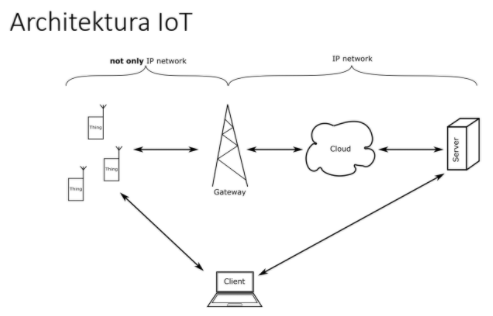
\includegraphics[width=0.6\linewidth]{S8.png}
	\caption{Krzywa ROC}
\end{figure}

\subsubsection{System autonomiczny - wyzwania}

\begin{itemize}
	\item prawa jednostki vs. prawa ogółu
	\item Social Credit System w Chinach
	\item prawa robotów (sztucznej inteligencji)
	\item prawo karne
	\item egzekwowanie
	\item zapobieganie
	\item prawo pracy
	\item prawo własności intelektualnej
	\item etyka
	\item ogromna ilość danych
	\item komunikacja
	\item przetwarzanie
	\item przechowywanie
	\item bezpieczeństwo
	\item zarządzanie infrastrukturą
	\item koszt energetyczny
	\item koszt
\end{itemize}

\subsubsection{Wyzwania technologiczne}

\begin{itemize}
	\item gromadzenie danych
	\begin{itemize}
		\item sensory
		\item sieci komunikacyjne
		\item przechowywanie
	\end{itemize}
	\item przetwarzanie danych
	\begin{itemize}
		\item dostępność
		\item algorytmy
	\end{itemize}
	\item autonomiczność pracy
	\begin{itemize}
		\item zasilanie
		\item niezawodność
	\end{itemize}
\end{itemize}

